\documentclass{article}

\usepackage{fancyhdr}
\usepackage{graphicx}
\usepackage{hyperref}

\headheight 24pt
\headsep 24pt
\pagestyle{fancy}

\linespread{1.3}

\begin{document}

\lhead{Tim Ekl}
\rhead{\textbf{MTM}}

\begin{center}
{\large \textbf{Mobile Trail Mapping}} \\
\textit{Exploring the Linn County, IA trails system}
\end{center}

Linn County, Iowa, is home to a significant trails system. Featuring over 30 miles of hiking, biking, and walking trails, Linn County trails are an important part of the larger Cedar Rapids recreational area.

The Linn County Trails Association (LCTA) is tasked with the maintenance of the trails, as well as publicity and mapping efforts for the system. In summer 2010, the LCTA decided to pursue a strategic redesign of their website, along with a push towards mobile technology to make the trails more accessible to the general public. It is with this mobile mapping effort that the LCTA requested Rose-Hulman's help; the result is Mobile Trail Mapping (MTM).

The MTM system is a cross-platform effort aimed at making up-to-date digital maps of the Linn County trails system available on multiple smartphone device types. At present, MTM applications exist for the iPhone and Android device ecosystems. Through a common server component, both platforms can access common trail data, including local points of interest (e.g. historical buildings, parking, restrooms, and so forth).

\subsubsection*{System features and requirements}

The LCTA wishes to maximize the value of the MTM applications to the Linn County populace. In addition, the Rose-Hulman team will be discontinuing work on the project in June 2011, and so LCTA staff will need to take over maintenance and administration of the system. With these constraints in mind, the LCTA laid down the following requirements for the MTM project:

\begin{itemize}
\item The project must provide mobile apps for both iPhone and Android platforms. These apps must present a common interface based on Google Maps which presents trail positions and relevant locations of interest. In addition, users should be able to submit data back to the server with information about trail problems. Finally, 
\item The project must allow authentication of users at different levels: registered users with the LCTA web site should see all data the system has to offer, while administrative users should be able to perform basic maintenance on trail data from the mobile device.
\item As the metropolitan population of Linn County exceeds a quarter million, the trail system must have reasonably high reliability. Downtime, while not business-critical, is contrary to the LCTA's mission.
\item The application and system should be free of charge and developed in an open, transparent manner.
\end{itemize}

With this in mind, the Rose-Hulman team designed a modern application architecture using public source control systems and Agile methodologies to fit the LCTA's needs.

\subsubsection*{MTM architecture and design}
The MTM architecture is based largely on two common software practices: Don't Repeat Yourself (DRY) and the Representational State Transfer (REST) pattern. The team quickly figured out it would be unnecessary to duplicate effort in implementing trail point information storage across both mobile platforms; instead, the trail data was abstracted to a common server application and provided to the mobile apps via XML. In this way, the project was kept DRY.

On the server, individual objects were maintained to represent each trail-related object (e.g. point, trail head, user, image). Each of these object implementations were provided with standard RESTful accessors to fetch and mutate the state of objects and their relationships. These accessors were centralized under a primary Ruby handler and run on the HostGator platform.

A primary concern in this network-based architecture was the reliance on wireless GPS and data transfer services. Though informal studies were performed to determine signal quality on the Linn County trails system, all aspects of the system had to be built in a fault-tolerant, caching manner in order to display the most seamless experience possible to the user.

On each mobile application, the architecture was fairly standard: using the provided libraries from the operating system providers (Apple and Google), the applications were written to query the server for data within the user's viewing window, then dynamically render the appropriate data. Each device used a passive caching strategy: data and images were stored locally, but a network connection was attempted whenever new data was to be loaded, and cache was only hit when no network data was available. This provided a balance between providing the user the most recent data for a given view and not relying too strongly on an available data connection.


\begin{center}
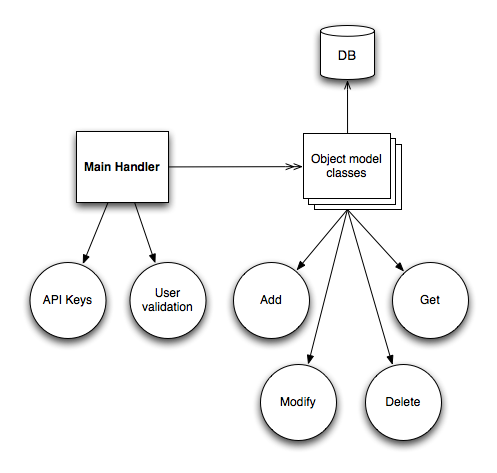
\includegraphics[width=4in]{../ArchitectureViews/server-components.png} \\
\textbf{Figure 1: Server architecture for the MTM applications}
\end{center}

\subsubsection*{Results and metrics}
The MTM applications were completed and delivered on time in mid-May 2011. Both queried against the \href{http://mtm.linncountytrails.org}{Linn County server} for all Linn County trail data. Overall, the project spanned over 300 files and 20,000 lines of code in 12 languages. The four developers of the project pushed over 1,200 commits to GitHub, the centralized source tracker used for MTM.

In addition to the completed website redesign, the MTM application provided a valuable addition to the Linn County trails portfolio and enhanced the trails for its users. Local users have also expressed interest in the platform; Rose-Hulman students, faculty, and staff have all proposed that the app be adapted for use during freshman orientation, for example. Overall, the MTM project has created a viable mobile mapping platform for a number of applications, as well as met (and even exceeded) the expectations of the LCTA.

\end{document}
